\section{Introduction}

The hardware nodes of a cloud service provider are often dedicated to running a single cloud service component.
%todo: think about cite something, e.g., facebook citation, and figure out if they actually use dedicated nature to do both, in which case we can combine above and next sentance
One hopes that this dedicated nature (i.e. fixed role in the service using a fixed software stack) can be exploited to obtain the required performance (e.g. 99\% tail latency) while minimizing the energy used (and thus the cost for providing the service). 
The importance of this task is magnified by the presence of increasingly constrained energy budgets in data centers~\cite{SmoothOperator, Dynamo, oldi}. 
%YA
When we consider the performance and energy use of a system, it is critical to note that they are emergent properties of the myriad of interactions between application software, operating systems, hardware, and offered loads.
However, if we then take a careful look at overall system execution under different energy profiles, we can see that the consequences of tuning energy and performance reach far beyond directly observable quantities and impact the interactions between the aforementioned system components in subtle ways.
%However, the performance and energy use of a system is an emergent property of the myriad of interactions between application software, operating systems, and hardware along with the offered load. 
%todo: above ends where, why is this a however?
%As OS developers do we really understand what is going on and the impact of each of our decisions?
Rather than focusing on the design and implementation of particular local or global mechanisms and policies for tuning performance and energy consumption, perhaps we need a greater understanding of their underlying impacts and dynamics.   

When designing and implementing an operating system, there is a dizzying array of mechanisms and policies one must consider, both at a local and global scale, that could both individually and collaboratively impact the performance and energy use of the system.
One must consider what should run after handling an interrupt and when should interrupts be enabled and disabled?
How should I/O-bound and CPU-bound work be identified and prioritized?
When should processors be put into sleep states and what sleep state should be used?
What values should processor energy settings be set to, should these values be dynamically adjusted, and if so, when and why?
What time constants should be used for various background tasks?
Should device settings be used to adjust their interrupt behaviour?
When and to what degree should polling versus interrupt-driven I/O be exploited and for which devices or logical streams?
If any settings should be exposed for manual adjustment or advice elicitation, should cooperative, preemptive, or hybrid scheduling be used?

Each of the above decisions can have both expected and unexpected impact on the realized performance and energy usage observed when the system is put into production, running particular applications and offered loads. 
Do the decisions we make have a significant impact on tuning the performance and energy consumption for network driven processing?  
%Do we understand the emergent interactions our software has with the hardware, application and the workload characteristics from this perspective?
Furthermore, does headroom exist for improving performance and energy consumption for dedicated processing, or can we at best expect to only trade one off for the other?
We have experimentally explored these questions and found the results fascinating, revealing both expected and unexpected results.


\begin{wrapfigure}{I}{.55\columnwidth}
\vspace{-0.5cm}
\centering
\begin{center}
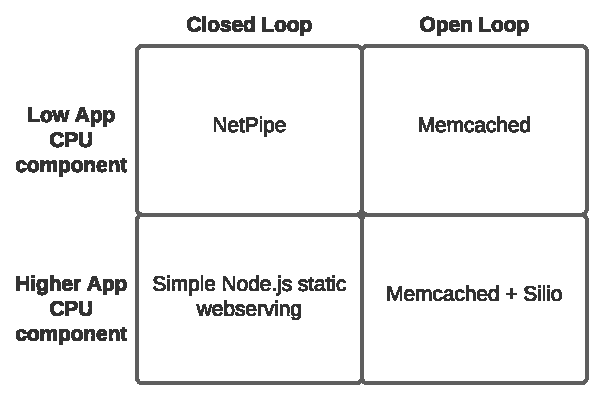
\includegraphics[width=.6\columnwidth]{figures/expgrid.pdf}
\vspace{-1cm}
\end{center}    
\end{wrapfigure}  


In this paper, we present findings from a detailed study of the emergent impact that server operating systems' design and implementation, as well as their interaction with hardware settings, can have on the combination of performance and energy.
We used four network-driven workloads to explore a grid of open and closed loop dynamics along with lower and higher application CPU requirements. 
With each workload, we ran thousands of experiments capturing detailed time series log data on every network interrupt.
This log data includes a high-precision timestamp, Joules consumed, instructions and cycles executed, sleep states entered, and last-level cache misses.
Each experiment has been run using both a general-purpose OS (Linux) and an application-specific Library OS (LicloseOS) and repeated across an exhaustive sweep of three hardware setting values: 1) Network Interface Card (NIC) Interrupt delay (ITR), 2) Dynamic Voltage and Frequency Scaling (DVFS) and 3) Running Average Power Limit (RAPL).
%We exhaustively sweep three hardware settings: 1) Network Interface Card (NIC) Interrupt delay (ITR), 2) Dynamic Voltage and Frequency Scaling (DVFS) and 3) Running Average Power Limit (RAPL) over both a general purpose OS (Linux) and an application specific Library OS (libOS).
Figures~\ref{fig:netpipe8Kov}-~\ref{fig:mcdsiloov} illustrate four of the energy-performance landscapes we observed.  
 
\begin{figure*}[t!]
\centering	
\begin{minipage}[t]{0.45\textwidth}
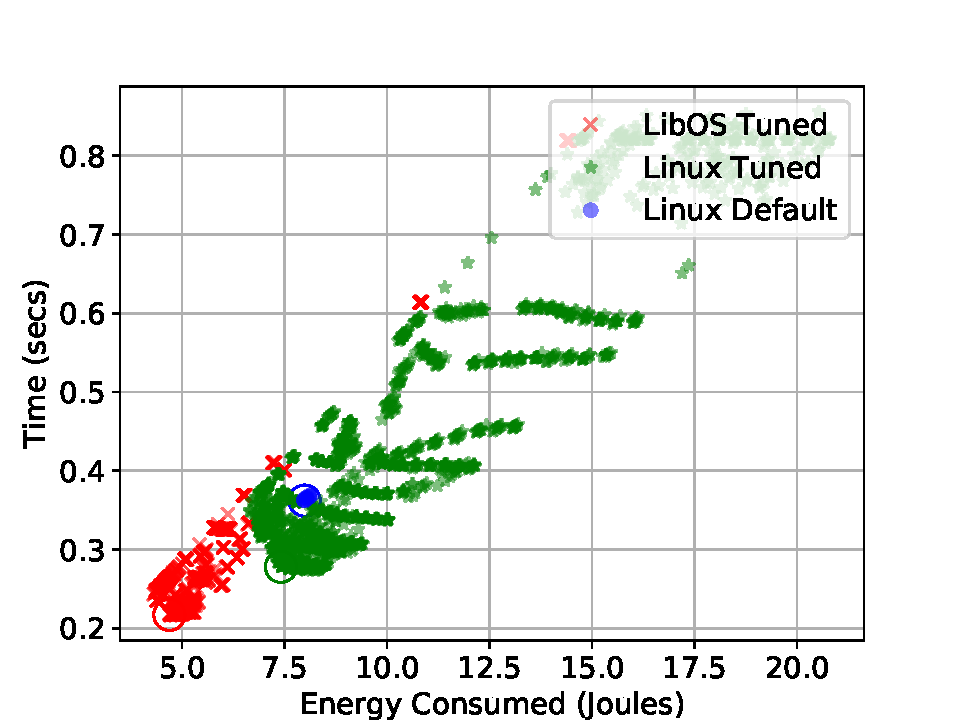
\includegraphics[width=\textwidth]{osdi_figures/netpipe_8192_overview.pdf}
	\caption{Netpipe 8KB overview}
	\label{fig:netpipe8Kov}
\end{minipage}
\begin{minipage}[t]{0.45\textwidth}
	\includegraphics[width=\columnwidth]{osdi_figures/mcd_600K_overview.pdf}
	\caption{Memcached 600K QPS}
	\label{fig:mcdov}
\end{minipage}
\begin{minipage}[t]{0.45\textwidth}
	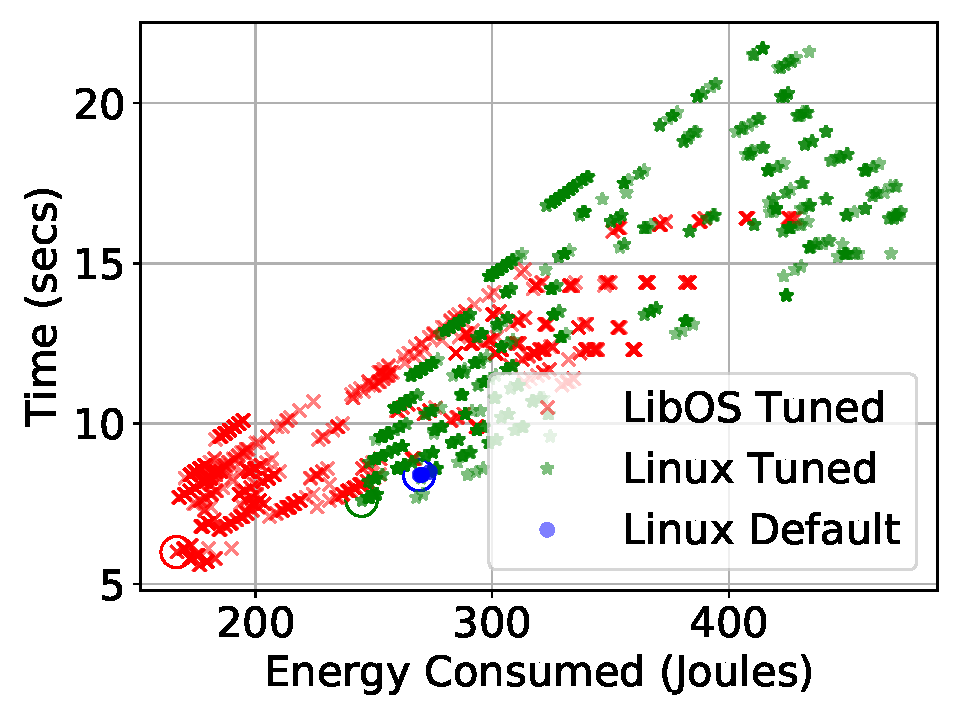
\includegraphics[width=\textwidth]{osdi_figures/nodejs_overview.pdf}
	\caption{NodeJS overview}
	\label{fig:nodejsov}
\end{minipage}
\begin{minipage}[t]{0.45\textwidth}
	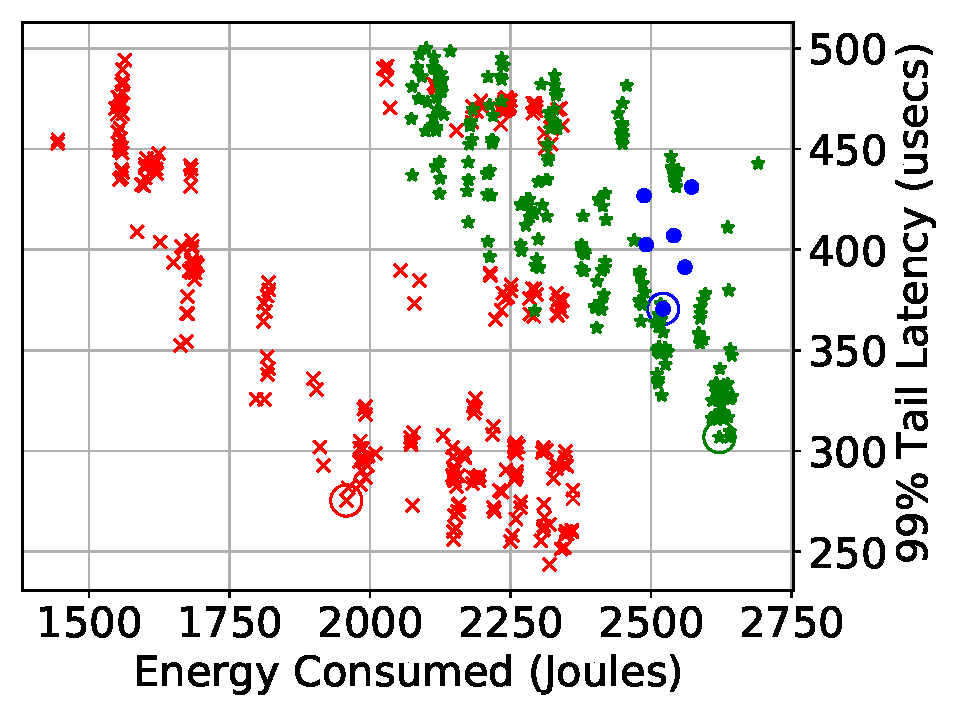
\includegraphics[width=\columnwidth]{osdi_figures/mcdsilo_200000_overview.pdf}
	\caption{MemCached Silo 200K QPS}
	\label{fig:mcdsiloov}
\end{minipage}
\end{figure*}
Each point in these graphs represents the results of an experimental run.
Using the log from each run, we calculate the total energy consumed along with a workload-specific measure.
In the case of netpipe and node.js workloads, the workload-specific measure we use is the time taken to complete some fixed number of sequential transactions in a closed-loop setting.
For netpipe (figure~\ref{fig:netpipe8Kov}), we measure the time taken to complete approximately 200,000 8Kb message round-trips between a client and server configured with the same OS and hardware settings.
For Node.JS (figure ~\ref{fig:nodejsov}), we measure the time required to serve 200,000 requests for a minimal static webpage.

In the case of the open-loop workloads Memcached and Memcached-Silo, we report the 99\% tail latency experienced while under a specific load of some number of queries-per-second (QPS) for a period of 20 seconds.
Specifically, for Memcached (figure~\ref{fig:itr_figure}), we apply an offered load of 600 QPS generated using the ETC Facebook benchmark~\cite{mutilate}.
For Memcached-Silo (figure~\ref{fig:mcdsiloov}), we apply a load of 200 QPS.
Note that, in both open-loop cases, the offered loads are close-to but do not exceed the system's capacity.
Furthermore, we filter any results that do not satisfy an SLA of 500 $\micro s$.  
Each experimental run uses a unique setting for the three hardware settings we study (ITR, DVFS, and RAPL) with each of the two OSs we consider.
We do not modify the OSs nor do we modify application software beyond choosing for Linux what is considered a production-quality configuration.

Each graph demonstrates the overall energy-versus-performance landscape that can be achieved for the given workloads and software bases considered.
Later sections of the paper present  details of how we conducted the experiments.
They focus on results for “optimal” points in these landscapes for both operating systems, whereby the hardware parameter settings brought about the best energy-performance tradeoff.
We also identify the results obtained when running the experiments on Linux using its default settings for these parameters.
The next section, however, discusses the landscape of hardware parameters more broadly and summarizes the core findings with respect to OS design and implementation.

%\vspace{2cm}

